\documentclass[a4paper]{article}
\usepackage{amsmath}  % Paquete necesario para \dfrac
\usepackage[utf8]{inputenc}
\usepackage[spanish]{babel}
\usepackage{graphicx}
\usepackage{array}
\usepackage{fancyhdr}
\usepackage{lastpage} % Paquete para obtener el número total de páginas
\usepackage{geometry} % Paquete para ajustar los márgenes
\usepackage[datesep=/,style=ddmmyyyy]{datetime2} % Paquete para formatear la fecha
\usepackage{setspace} % Incluye el paquete setspace
\usepackage{enumitem}
\usepackage{amssymb} % Para más símbolos
\usepackage{indentfirst}
\usepackage{hyperref}
\usepackage{array}
\usepackage{booktabs}

\usepackage{titlesec} % Incluye el paquete titlesec
% Redefiniendo el formato del título de la sección con un tamaño de fuente más pequeño
\titleformat{\section}
{\normalfont\large\bfseries}{\thesection}{1em}{}

% Definiendo los márgenes de la página y del encabezado
\geometry{
	left=20mm,
	right=20mm,
	top=40mm,
	bottom=30mm,
	headsep=20mm
}

\pagestyle{fancy}
\fancyhf{} % Limpia el encabezado y pie de página predeterminados
\renewcommand{\headrulewidth}{0pt} % Elimina la línea del encabezado
\renewcommand{\footrulewidth}{0.4pt} % Línea sobre el pie de página

\fancyhead[C]{ % Contenido centrado en el encabezado
	\begin{tabular}{|m{3.5cm}|m{9.0cm}|m{3.5cm}|}
		\hline
		\begin{minipage}[c][2.0cm][c]{3.5cm}
			\centering
			
\includegraphics[width=2.98cm,height=1.25cm]{logo.png}
		\end{minipage} & 
		\begin{minipage}[c][2.0cm][c]{9cm}
			\centering
			\hyphenpenalty=10000 % Evita la separación de palabras
			\vspace*{\fill} % Espacio vertical flexible antes del texto
			\begin{spacing}{1.5} % Aumenta el espacio entre líneas a 1.25
				{\large \textbf{Inductor para la Reducción de la Corriente Transitoria \textit{Inrush} en Condensadores}}
			\end{spacing}
			\vspace*{\fill} % Espacio vertical flexible después del texto
		\end{minipage} & 
		\begin{minipage}[c][2.0cm][c]{3.5cm}
			\raggedleft
			Emisión: \DTMtoday \\
			Página: \thepage/\pageref{LastPage}
		\end{minipage} \\
		\hline
	\end{tabular}
}

% Contenido del pie de página
\fancyfoot[L]{%
	\begin{tabular}[b]{@{}l@{}}
		\href{http://www.dax.energy}{www.dax.energy}
	\end{tabular}
}
\fancyfoot[C]{%
	\begin{tabular}[b]{@{}c@{}}
		\href{mailto:comercial@dax.energy}{comercial@dax.energy}
	\end{tabular}
}
\fancyfoot[R]{%
	\begin{tabular}[b]{@{}r@{}}
		+55 41 99940-3744 \\ 3626-2072
	\end{tabular}
}

\begin{document}
	\setstretch{1.25} % Define el espacio entre líneas en 1.25
	
	\section{Contexto}
	La energización de un banco de condensadores (Figura \ref{fig:picture1}) mediante el cierre de un disyuntor resultará en una alta corriente de pico transitoria (Figura \ref{fig:picture2}), denominada inrush. La magnitud y frecuencia de esta corriente de pico transitoria son funciones de:
	\begin{itemize}[label=\textendash]
		\item el voltaje aplicado (punto en la onda de voltaje en el momento del cierre);
		\item la capacitancia equivalente del circuito;
		\item la inductancia en el circuito (cantidad y ubicación);
		\item la carga en el banco de condensadores en el momento del cierre;
		\item cualquier amortiguamiento del circuito debido a resistencias de cierre u otra resistencia en el circuito.
	\end{itemize}
	
	\section{Datos de entrada del banco}
	\begin{itemize}[label=\textendash]
		\item Potencia reactiva  = 27.0 MVAr
		\item Voltaje trifásico  = 13.8 kV
		\item Voltaje monofásico  = 8.0 kV
		\item Corriente de cortocircuito  = 20.0 kA
	\end{itemize}
	
	\begin{center}
		\begin{tabular}{lllllllllll}
\toprule
 & $Q_{3\phi}$ & $Q_{1\phi}$ & $V_{3\phi}$ & $V_{1\phi}$ & $I_{1\phi}$ & $X_{1\phi}$ & $C_{1\phi}$ & $L_{1\phi}$ & $I_{p}/I_{n}$ & $f_{0}$ \\
\midrule
0 & 5.4 MVAr & 1.8 MVAr & 13.8 kV & 8.0 kV & 225.9 A & 35.3 $\Omega$ & 75.22 µF & 15.0 µH & 13.0 & 559.3 Hz \\
1 & 5.4 MVAr & 1.8 MVAr & 13.8 kV & 8.0 kV & 225.9 A & 35.3 $\Omega$ & 75.22 µF & 15.0 µH & 47.9 & 4.1 kHz \\
2 & 5.4 MVAr & 1.8 MVAr & 13.8 kV & 8.0 kV & 225.9 A & 35.3 $\Omega$ & 75.22 µF & 15.0 µH & 64.0 & 4.1 kHz \\
3 & 5.4 MVAr & 1.8 MVAr & 13.8 kV & 8.0 kV & 225.9 A & 35.3 $\Omega$ & 75.22 µF & 15.0 µH & 72.0 & 4.1 kHz \\
4 & 5.4 MVAr & 1.8 MVAr & 13.8 kV & 8.0 kV & 225.9 A & 35.3 $\Omega$ & 75.22 µF & 15.0 µH & 76.8 & 4.1 kHz \\
\bottomrule
\end{tabular}

	\end{center}
	
	\section{Consideraciones iniciales}
	
	La corriente \textit{inrush} transitoria no es un factor limitante en aplicaciones de bancos de condensadores aislados. Sin embargo, cuando los bancos de condensadores se conmuten \textit{back-to-back}, es decir, cuando se activa un banco mientras otro banco está conectado al mismo barraje, fluirán corrientes transitorias de alta magnitud y frecuencia natural entre el banco activado y los que ya estaban activados.
	
	\begin{figure}[!hbp]
		\centering
		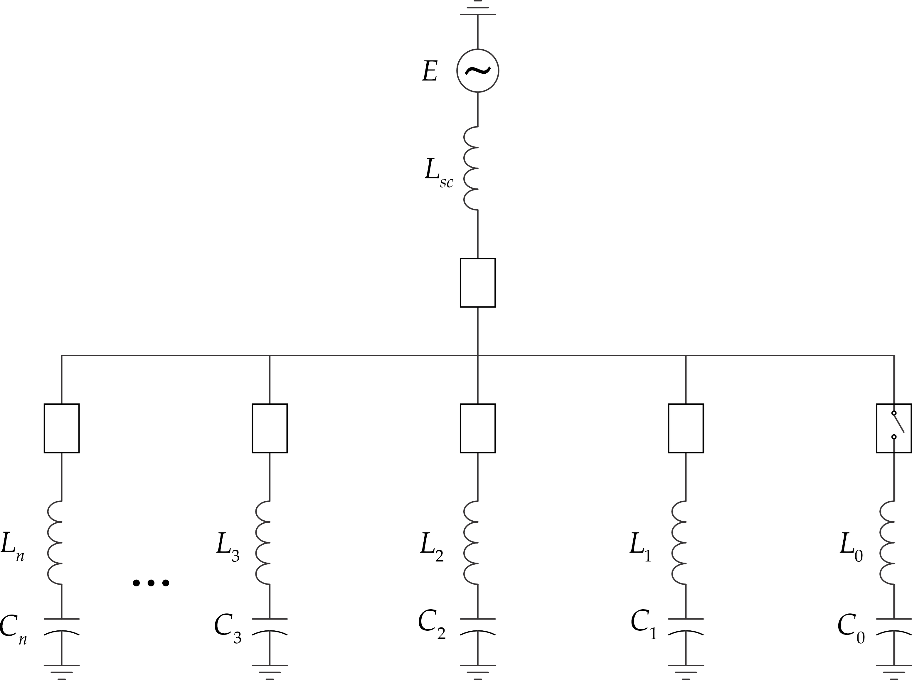
\includegraphics{Picture1.png}
		\caption{Sistema de banco de condensadores.}
		\label{fig:picture1}
	\end{figure}
	
	Esta corriente oscilatoria está limitada únicamente por la impedancia del banco de condensadores y el circuito entre los bancos energizados y el banco conmutado (Banco \#0), que generalmente decae a cero en una fracción de un ciclo de la frecuencia del sistema. En el caso de la conmutación \textit{back-to-back}, el componente proporcionado por la fuente está en una frecuencia más baja (60 Hz) y es tan pequeño en comparación con la corriente \textit{inrush} que puede ser despreciado \href{https://ieeexplore.ieee.org/document/7035261}{[ANSI/IEEE C37.012-1979]}.
	
	\section{Resultados}
	\begin{figure}[!hbp]
		\centering
		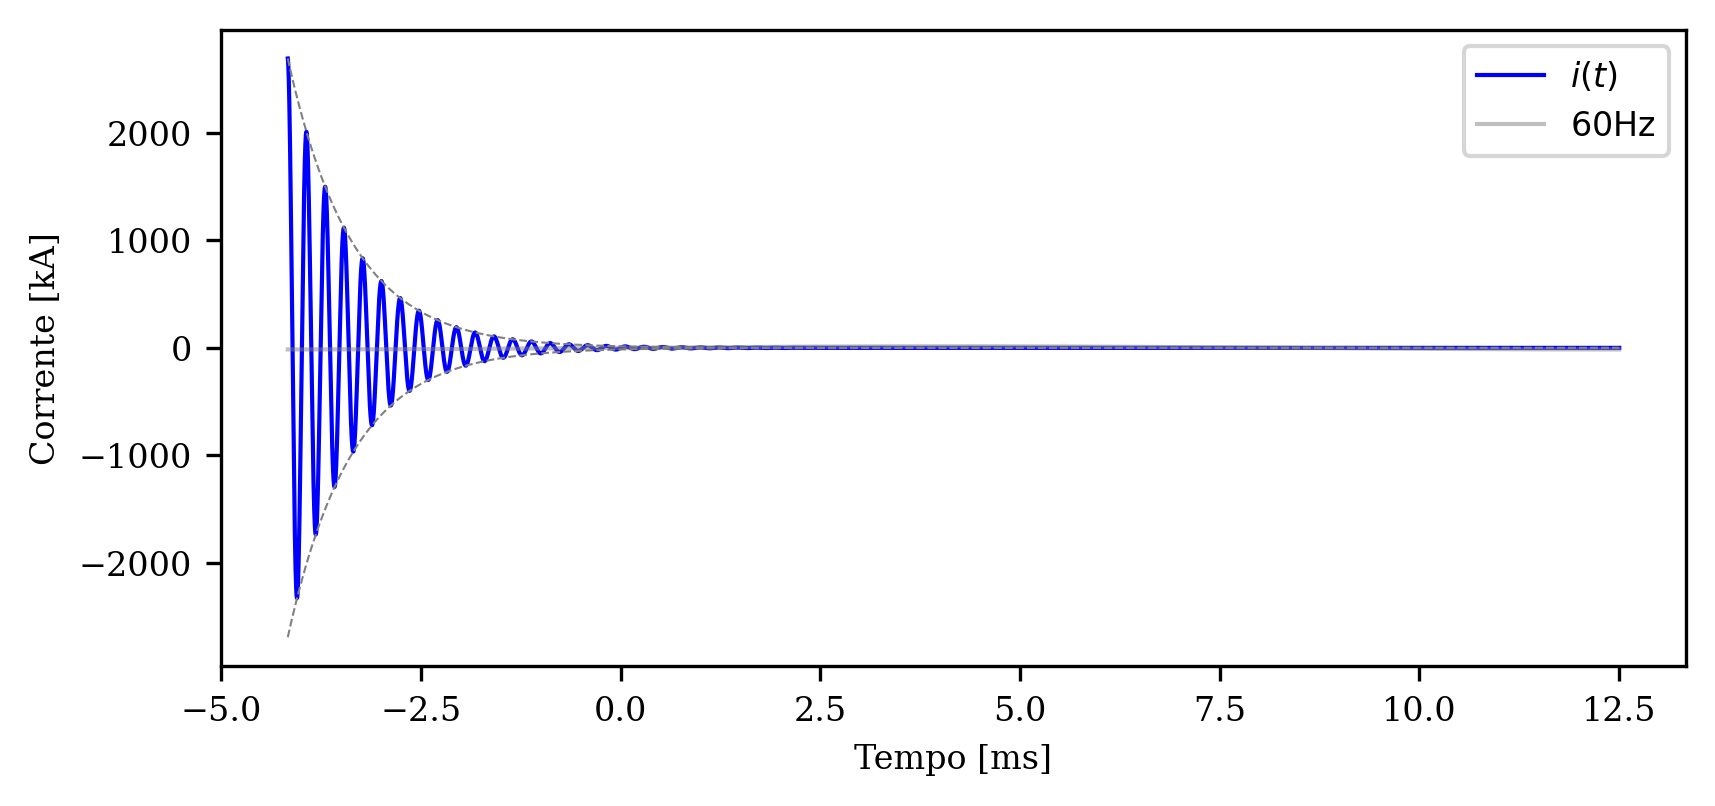
\includegraphics{Correntes.png}
		\caption{Corriente instantánea en el banco de condensadores activado en un ciclo de la frecuencia fundamental.}
		\label{fig:picture2}
	\end{figure}
	
	Los valores obtenidos con el reactor seleccionado ($L_{reator} = 15.0 \, \mu \rm{H} $) son:
	\begin{itemize}[label=\textendash]
		\item Corriente de pico: 24.5 kA;
		\item Frecuencia de oscilación: 4.1 kHz;
		\item Corriente inrush / Corriente nominal: 76.8
	\end{itemize}
	
	\section{Conclusión}
	Reactor adecuado, ya que $\dfrac{I_{\rm inrush}}{I_{\rm rated}} = $76,83$\le 100$ e $f_{\rm osc} = $4,091,12Hz < 4,25 kHz, IEEE Std C37.012, p. 16[$^{[2]}$](https://ieeexplore.ieee.org/document/7035261) e IEC 62271-100, Table 9 (Preferred values of rated capacitive switching currents), p. 45[$^{[3]}$](https://webstore.iec.ch/publication/62785).
	
	\section{Referencias}
	
	\noindent
	\begin{tabular}{p{0.2cm} p{15.8cm}}
		\href{https://ieeexplore.ieee.org/document/7035261}{[1]} &
		\begin{minipage}[t]{15.8cm}
			Guía de aplicación IEEE para la conmutación de corriente de capacitancia para interruptores automáticos de alta tensión AC clasificados en una base de corriente simétrica, en ANSI/IEEE C37.012-1979, vol., no., pp.1-54, 6 Feb. 1979, doi: 10.1109/IEEESTD.1979.7035261.
		\end{minipage} \\
		
		\href{https://ieeexplore.ieee.org/document/9574631}{[2]} &
		\begin{minipage}[t]{15.8cm}
			Proyecto de norma aprobado por IEEE para los requisitos de interruptores de condensadores para sistemas AC (1 kV a 38 kV), en IEEE PC37.66/D10, octubre de 2021, vol., no., pp.1-35, 13 Dic. 2021.
		\end{minipage} \\
		
		
		\href{https://webstore.iec.ch/publication/62785}{[3]} &
		\begin{minipage}[t]{15.8cm}
			Interruptores y equipos de control de alta tensión IEC 62271-100 - Parte 100: Interruptores automáticos de corriente alterna
		\end{minipage} \\
		
    \href{https://ieeexplore.ieee.org/document/5318709}{[4]} &
\begin{minipage}[t]{15.8cm}
	Norma IEEE para interruptores automáticos de alta tensión AC clasificados en una base de corriente simétrica: Valores preferidos y capacidades requeridas relacionadas para tensiones superiores a 1000 V, en IEEE Std C37.06-2009, vol., no., pp.1-56, 6 Nov. 2009, doi: 10.1109/IEEESTD.2009.5318709.
\end{minipage} \\

\href{https://cdn.standards.iteh.ai/samples/101972/4e7e06bd66d2443da668b8e0c6c60512/IEC-62271-100-2021.pdf}{[5]} &
\begin{minipage}[t]{15.8cm}
	Interruptores y equipos de control de alta tensión IEC 62271-100 – Parte 100: Interruptores automáticos de corriente alterna.
\end{minipage} \\

\href{https://www.normas.com.br/autorizar/visualizacao-nbr/313/identificar/visitante}{[6]} &
\begin{minipage}[t]{15.8cm}
	NBR 5282 Condensadores de potencia en derivación para sistemas de tensión nominal superior a 1000 V.
\end{minipage} \\
\end{tabular}

% Espacio para firmas
\noindent % Evita la sangría
\begin{minipage}[t]{0.5\textwidth} % Comienza la primera columna para la firma
\centering % Alinea el texto al centro
\vspace{5cm} % Espacio reservado para la firma
\rule{6cm}{0.4pt}\\ % Línea para la firma
\textbf{Angelo A. Hafner}\\ % Nombre
Ingeniero Eléctrico\\ % Título
CONFEA: 2.500.821.919\\ % Número de registro
CREA/SC: 045.776-5\\ % Otro número de registro
aah@dax.energy % Correo electrónico
\end{minipage}%
\hfill % Espacio entre las columnas
\begin{minipage}[t]{0.5\textwidth} % Comienza la segunda columna para la firma
\centering % Alinea el texto al centro
\vspace{5cm} % Espacio reservado para la firma
\rule{6cm}{0.4pt}\\ % Línea para la firma
\textbf{Tiago Machado}\\ % Nombre
Gerente de Negocios\\ % Título
Mobile: +55 41 99940-3744\\ % Contacto
tm@dax.energy % Correo electrónico
\end{minipage}

\end{document}

